\lstinputlisting[language=bash,basicstyle=\small]{python_codes/fieldstone_106/keywords}

\begin{center}
Code at \url{https://github.com/cedrict/fieldstone/tree/master/python_codes/fieldstone_106}
\end{center}

\par\noindent\rule{\textwidth}{0.4pt}

%%%%%%%%%%%%%%%%%%%%%%%%%%%%%%%%%%%%%%%%%%%%%%%%%%%%%%%%%%%%%%%%%%%%%%%%%%%%%%%%%%%%%%%%%%%%%%%%%%%%


This stone is inspired by Kellogg \& King (1997) \cite{keki97}. 

\begin{center}
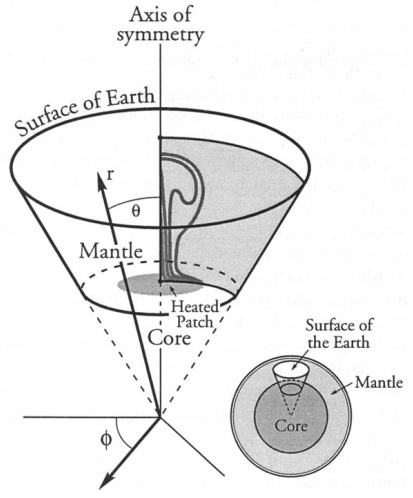
\includegraphics[width=6cm]{python_codes/fieldstone_106/images/keki97a}\\
{\captionfont Taken from \cite{keki97}.}
\end{center}

I set out to reproduce the results of the original publication. 
The necessary information is spread out throughout the first pages.
In Section~3 it is stated that the angular opening is $\pi/4$ and $r_i/r_o=0.55$.
However, it is not clear what $r_i$ or $r_o$ are, although Section~3
mentions $r$ values of 1.7 which is somewhat in the 'middle' of the cone. 
Because the equations in the paper are in dimensionless form, and 
because it is common to choose the depth of the mantle as reference length, 
then we probably have $r_o-r_i=1$. In this case we find $r_i=1.22\dots$ and 
$r_o=2.22\dots$ ({\color{orange} 1st guess}: confirmed by S.K., June 2021).

Free-slip boundary conditions are imposed on all boundaries.
A patch on the inner boundary of the shell was heated by
maintaining it at a constant dimensionless temperature of $T_{patch}=1$; 
elsewhere the base of the shell was insulating ($\partial T/\partial r = 0$).
At the top of the shell, a constant dimensionless temperature of $T_{top}=0$ was maintained.
Unfortunately it is not specified how wide the patch is, so I choose 
$\pi/8$ which seems probable when looking at Figure~3 ({\color{orange} 2nd guess}: confirmed by S.K., June 2021).
The sides of the cone were insulating ($\partial T/\partial \theta =0$).
Because of how FE works the insulating boundary conditions are automatically enforced 
when Dirichlet boundary conditions are absent. 

The rheology is temperature-dependent viscous:
\[
\eta(T) =\eta_0 \exp\left[ E \left( \frac{1}{T+T_0} -\frac{1}{1+T_0}  \right)   \right]
\]
with $E= \{0,0.25328,3\}$. $T_0$ is defined as ``the surface temperature divided by the temperature
drop across the shell'' but its value is not specified. On earth the surface temperature is $\sim300\si{\kelvin}$
while the temperature drop across the mantle is $\sim3000\si{\kelvin}$ 
so I take $T_0=0.1$ ({\color{orange} 3rd guess}: S.K. says that $\Delta T$ can be recovered from the Rayleigh number and using standard Earth values for all other parameters, but given the uncertainty about the Rayleigh number itself, this parameter is lost forever.).
The value for $\eta_0$ is also not specified but if this value is used as reference viscosity value 
during the adimensionalisation process then $\eta_0=1$ ({\color{orange} 4th guess}).
The initial temperature in the domain is set to $T=0.25$.

As seen in Section~\ref{XYZ}, the dimensionless heat transport equation is void of any coefficient is 
$\kappa/h$ is used as a reference velocity (where $h$ is a reference length) so we take the 
dimensionless value of $\kappa$ to be 1.   

Looking at Eq.~1 we find that there probably is a factor 2 missing before 
the viscosity $\mu$ ({\color{orange} 5th guess}: confirmed by S.K., June 2021).
In Section~2.2 it is stated that the SUPG method is used (see Section~\ref{YUG}) but how the stabilisation parameter
is chosen is not specified ({\color{orange} 6th guess}).

In the end the set of equations solved by the code is as follows:
\begin{eqnarray}
-\vec\nabla p + \vec\nabla \cdot(2 \eta \dot{\bm \varepsilon} ) &=& \Ranb \; T \vec{e}_r \\
\vec\nabla\cdot\vec\upnu &=& 0 \\
\frac{\partial T}{\partial t} + \vec\upnu\cdot\vec\nabla T &=& \Delta T 
\end{eqnarray}
Given the above boundary conditions, initial temperature and Rayleigh number value $\Ranb=10^7$ these
equations can be solved. 

Concerning the value of $\Ranb$, it is said to be $10^7$ but preliminary runs (in 2D) yield much 
narrower plumes for the isoviscous case than in the paper. However using $10^6$ 
instead seems to visually match the paper's results. I asked S.K. whether 
there could not be a mistake in the reported Ra in the paper and he kindly answered the following:
"A mistake is always possible. Here’s a possibility, the $\Ranb=10^7$ was what was input into the 
input file but we did not do a proper internal scaling to account for this, i.e. 
$r_o^3$ was used rather than $(r_o-r_i)^3$ with $r_o^3 = 2.22^3 \sim 10$.  
Usually in our codes what we put in as the Rayleigh number is really rho-g-alpha and all the other factors are 
input as 1 (or implicitly assumed to be 1).  
At any rate, I suspect $10^6$ could be a result of not accounting properly for the radius not being 1.0.  
I found some files one of my students used circa 2007 and the Ra was set to $10^7$ in the input file 
while the grid (different file) was $1.2 \rightarrow 2.2$.  I could see how one would forget 
when it comes to writing up the paper."

The paper does mention dimensioned quantities twice: in the caption of Fig.~3, we 
learn that 
$t=0.000561$ corresponds to $1.5\cdot 10^8\si{\year}$,
$t=0.000730$ corresponds to $2.0\cdot 10^8\si{\year}$, and
$t=0.016353$ corresponds to $4.4\cdot 10^9\si{\year}$.
This yields a reference time of about 270e9, which is close 
to ours $t_{ref}=h^2/\kappa = (2891e3)^2/10^{-6}\sim 8.36\cdot 10^{18}s \sim 265\cdot 10^9 \si{\year}$.


The code relies on $Q_2\times Q_1$ elements. The user chooses the number of elements in the 
radial direction $nelr$ and the number of elements in the tangential direction is automatically 
computed as $nelt=1.5\cdot nelr$.
Elements on the boundaries are flagged by means of the $flag\_el\_X$ array ($X=1,2,3,4$ 
corresponding to left, right, bottom and top). 
Similar boolean arrays are setup for nodes on the boundaries: $flag\_X$. 
Free-slip boundary conditions are more difficult to impose than for Cartesian domains 
because the boundaries of the computational domain are either curved and/or not aligned
with the Cartesian axis. 
The timestep is computed by means of a CFL criterion, but it is limited to a $2\times$ 
increase from one time step to the next to insure a somewhat smooth transition at 
the beginning when the plume is rising faster and faster.


\begin{remark}
At the moment the code is 2D, not axisymmetric!
LK filter and/or SUPG should be tested (at the moment the temperature us thresholded in the 
material model). Explore resolution, initial T in the mantle, try scaled-down Steinberger average 
viscosity profile, look at dynamic topography, strain-rate dependent power-law rheology, different 
Ra number, ... finish scaling up to real Earth like dimensions.
Would be nice to normalise the pressure on the top surface, not only a corner.
Also remove all bc on sides and use reduced density only? 
\end{remark}



\newpage
%%%%%%%%%%%%%%%%%%%%%%%%%%%%%%%%%%%%%%%%%%%%%%%%%%%
\subsubsection*{Isoviscous model}

In this case $E=0$ so the uncertainty about $T_0$ is irrelevant. The other ones do remain.

\begin{center}
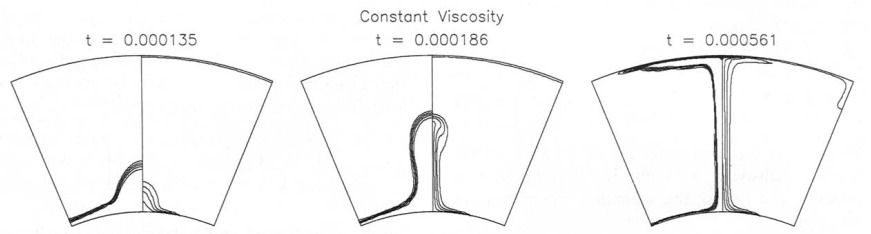
\includegraphics[width=15cm]{python_codes/fieldstone_106/images/keki97b}
\end{center}

The following results obtained on various meshes. No SUPG. CFL number is 1. Q2Q1 elements. $\Ranb=10^6$. 

\begin{center}
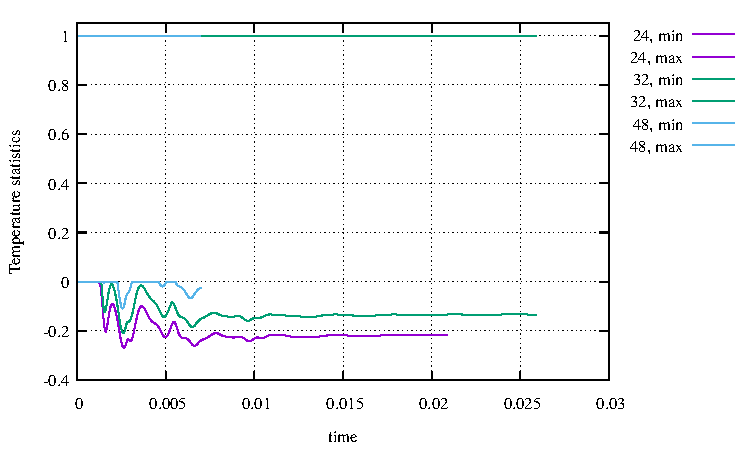
\includegraphics[width=7cm]{python_codes/fieldstone_106/results/exp1/stats_T.pdf}
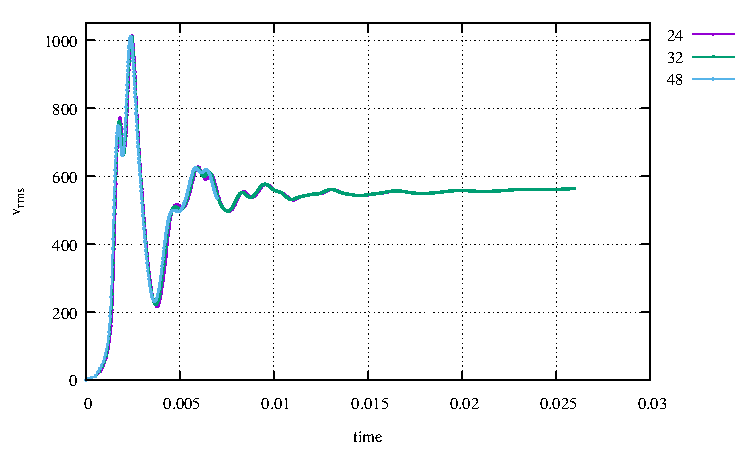
\includegraphics[width=7cm]{python_codes/fieldstone_106/results/exp1/vrms.pdf}\\
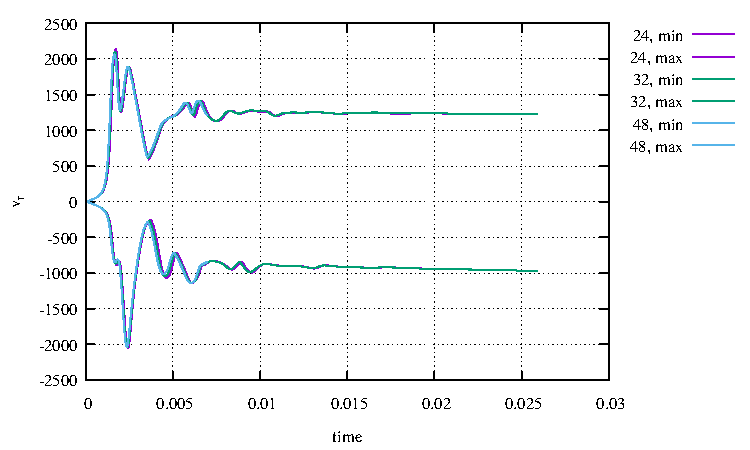
\includegraphics[width=7cm]{python_codes/fieldstone_106/results/exp1/stats_vr.pdf}
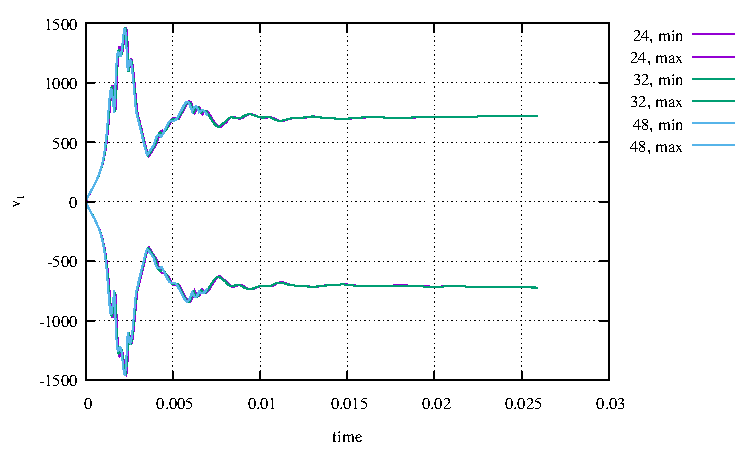
\includegraphics[width=7cm]{python_codes/fieldstone_106/results/exp1/stats_vt.pdf}\\
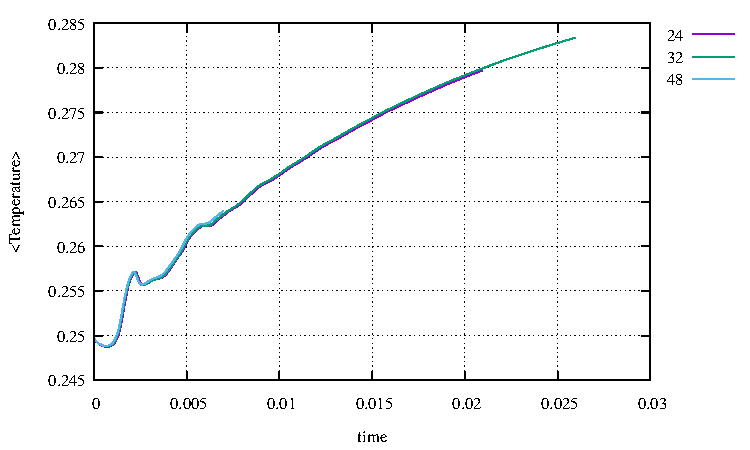
\includegraphics[width=7cm]{python_codes/fieldstone_106/results/exp1/Tavrg.pdf}
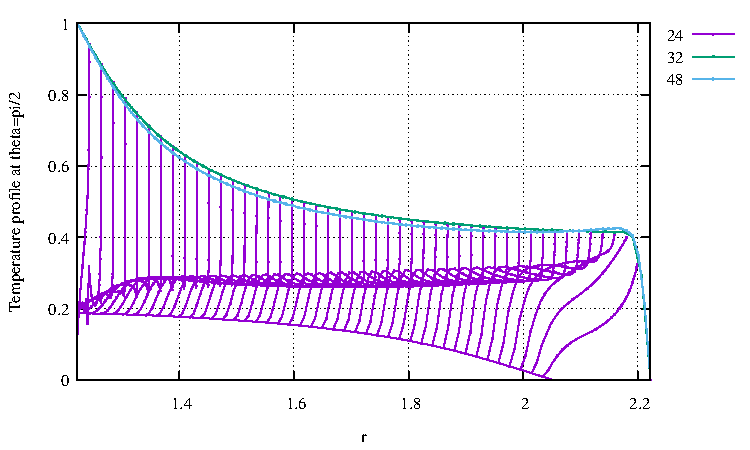
\includegraphics[width=7cm]{python_codes/fieldstone_106/results/exp1/profile_T.pdf}\\
{\captionfont Note that none of the runs actually reached steady state. Also 
profiles are therefore not reliable.} 
\end{center}
We find that results agree rather well between resolutions.

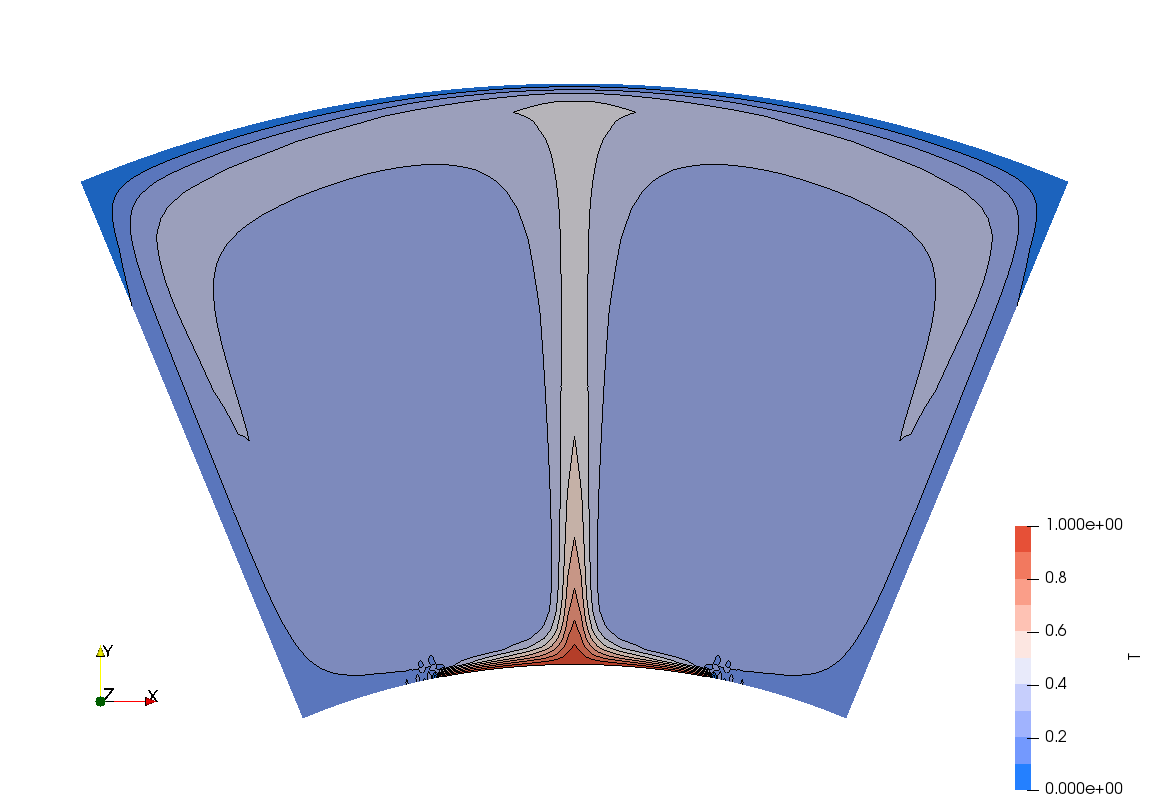
\includegraphics[width=5cm]{python_codes/fieldstone_106/results/exp1/nelr32/T}
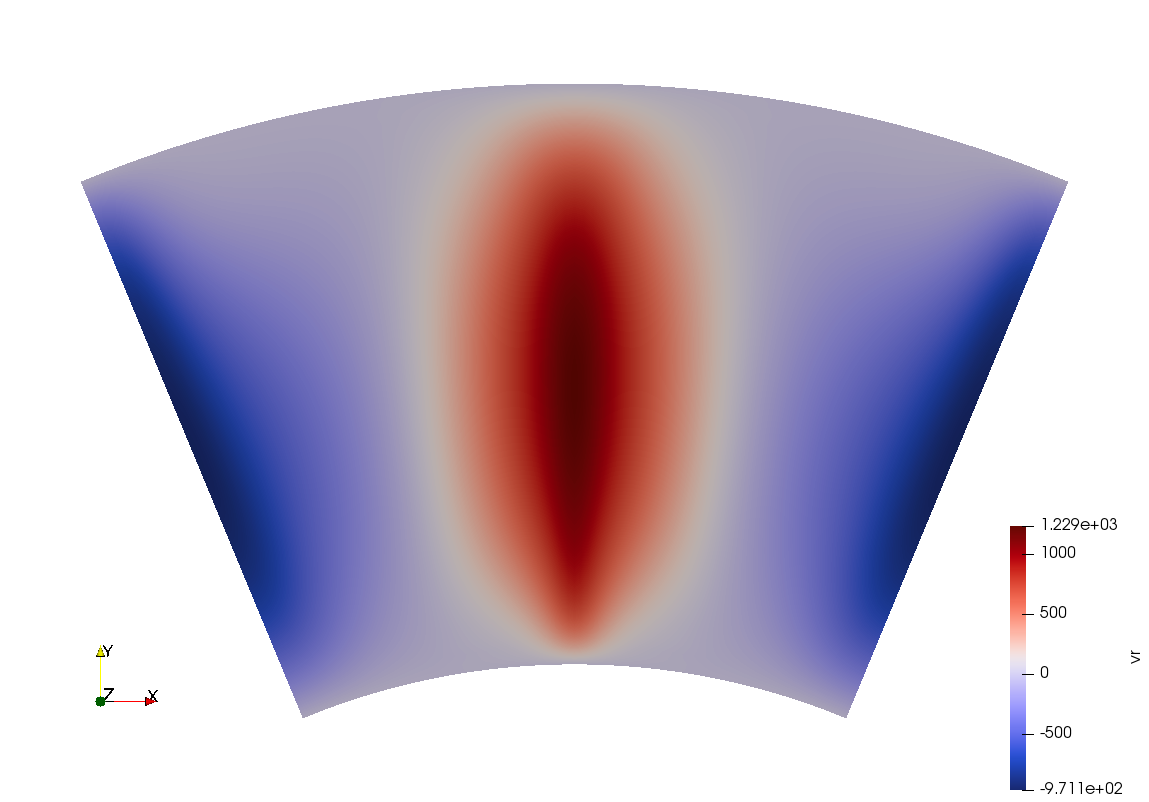
\includegraphics[width=5cm]{python_codes/fieldstone_106/results/exp1/nelr32/vr}
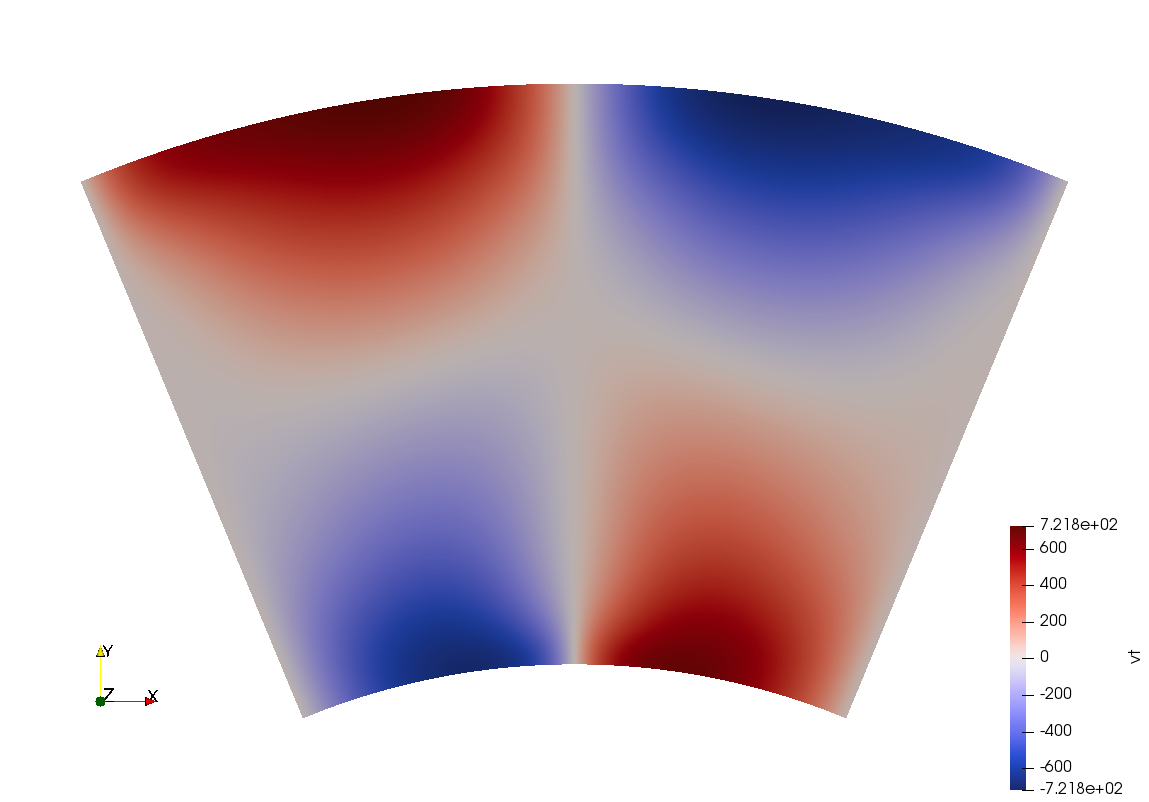
\includegraphics[width=5cm]{python_codes/fieldstone_106/results/exp1/nelr32/vt}

\newpage
%%%%%%%%%%%%%%%%%%%%%%%%%%%%%%%%%%%%%%%%%%%%%%%%%%%
\subsubsection*{Weakly temperature-dependent model}
\begin{center}
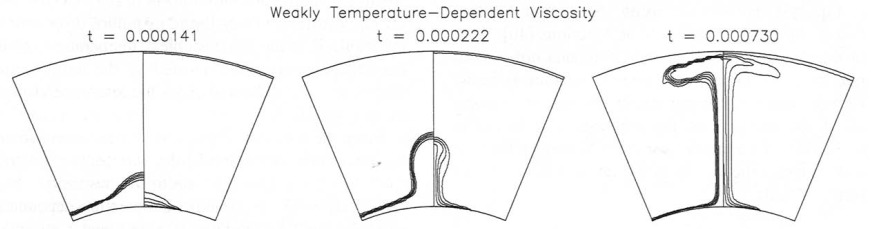
\includegraphics[width=15cm]{python_codes/fieldstone_106/images/keki97c}
\end{center}

\begin{center}
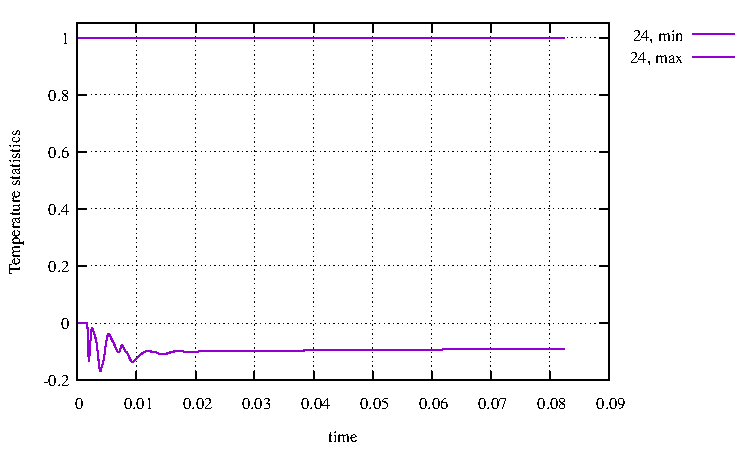
\includegraphics[width=5cm]{python_codes/fieldstone_106/results/exp2/stats_T.pdf}
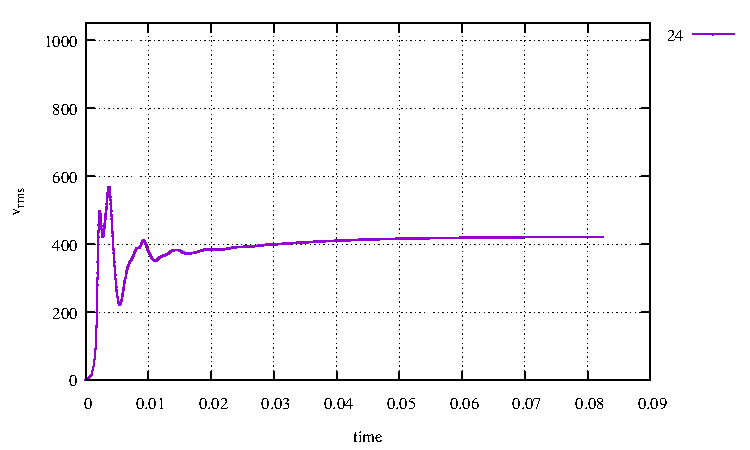
\includegraphics[width=5cm]{python_codes/fieldstone_106/results/exp2/vrms.pdf}\\
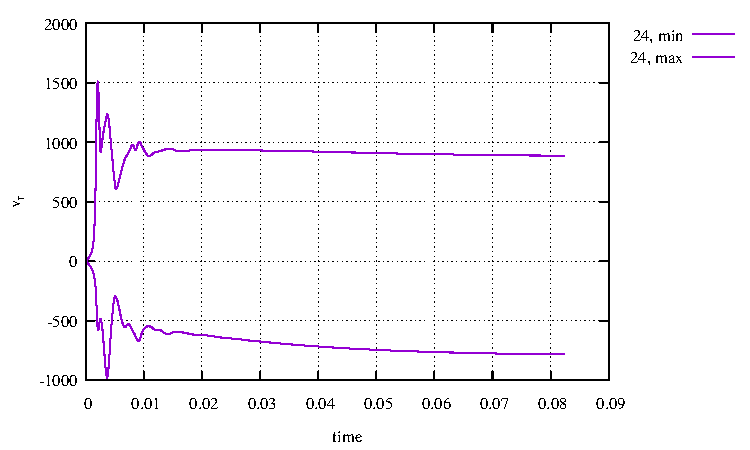
\includegraphics[width=5cm]{python_codes/fieldstone_106/results/exp2/stats_vr.pdf}
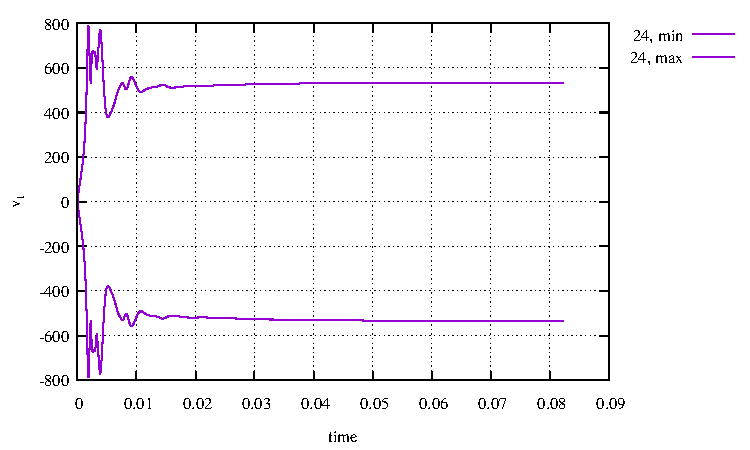
\includegraphics[width=5cm]{python_codes/fieldstone_106/results/exp2/stats_vt.pdf}\\
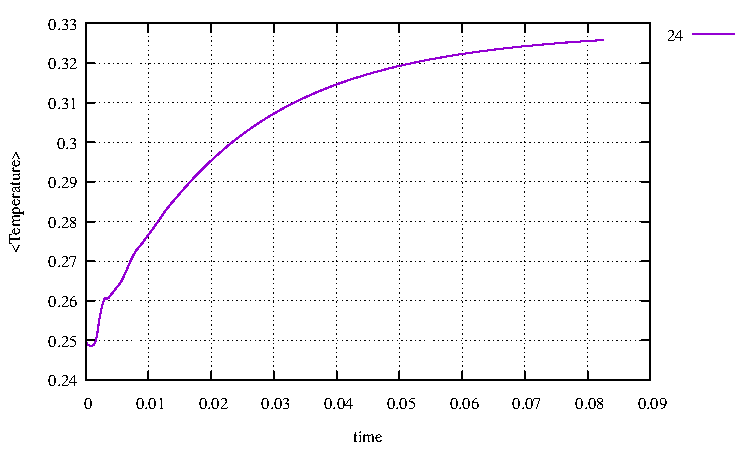
\includegraphics[width=5cm]{python_codes/fieldstone_106/results/exp2/Tavrg.pdf}
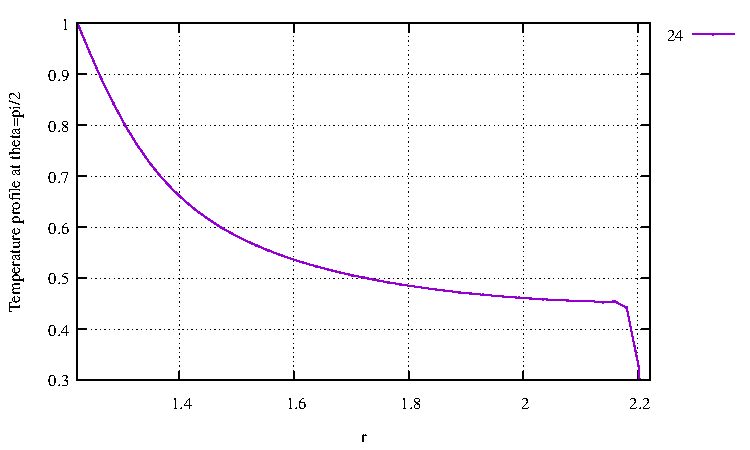
\includegraphics[width=5cm]{python_codes/fieldstone_106/results/exp2/profile_T.pdf}\\
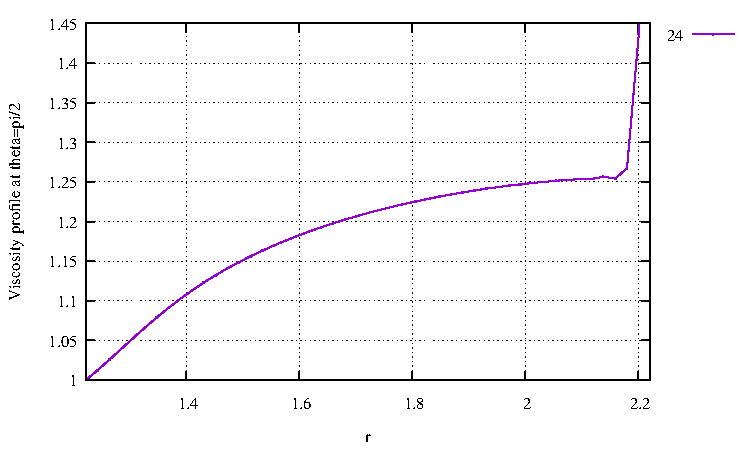
\includegraphics[width=5cm]{python_codes/fieldstone_106/results/exp2/profile_eta.pdf}\\
{\captionfont Note that none of the runs actually reached steady state. Also 
profiles are therefore not reliable.} 
\end{center}

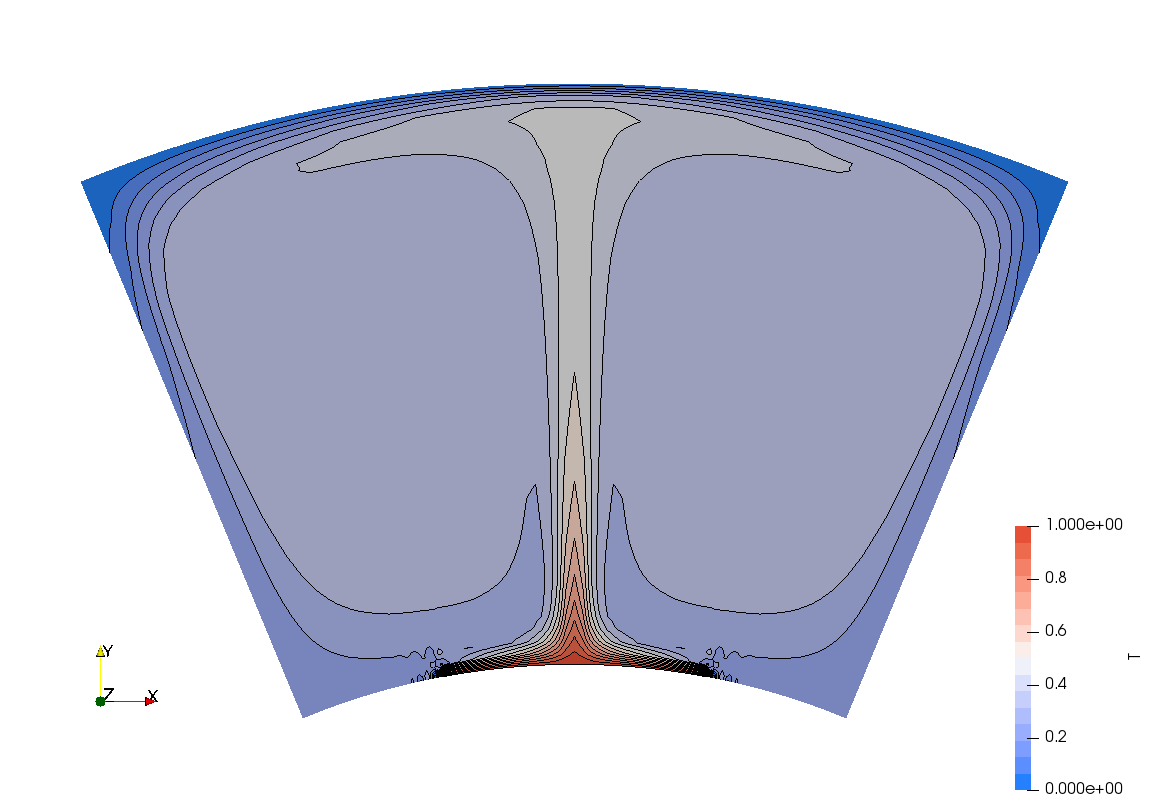
\includegraphics[width=5cm]{python_codes/fieldstone_106/results/exp2/nelr24/T}
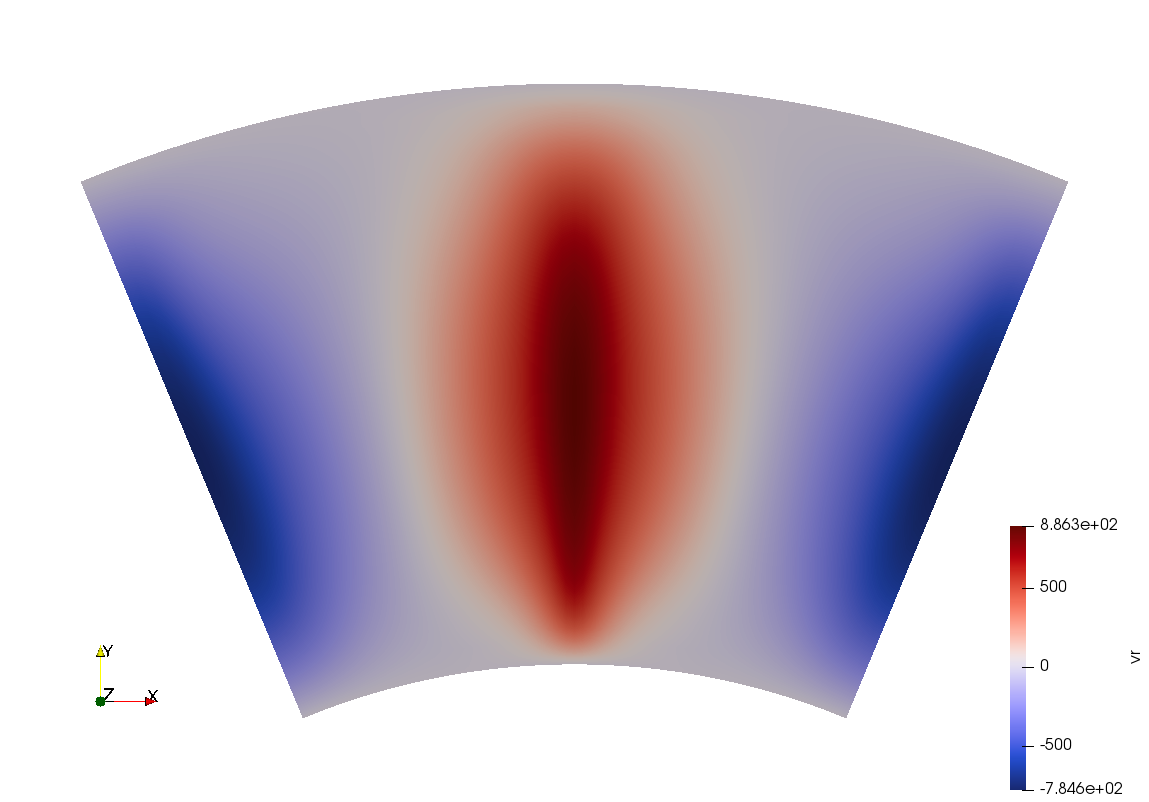
\includegraphics[width=5cm]{python_codes/fieldstone_106/results/exp2/nelr24/vr}
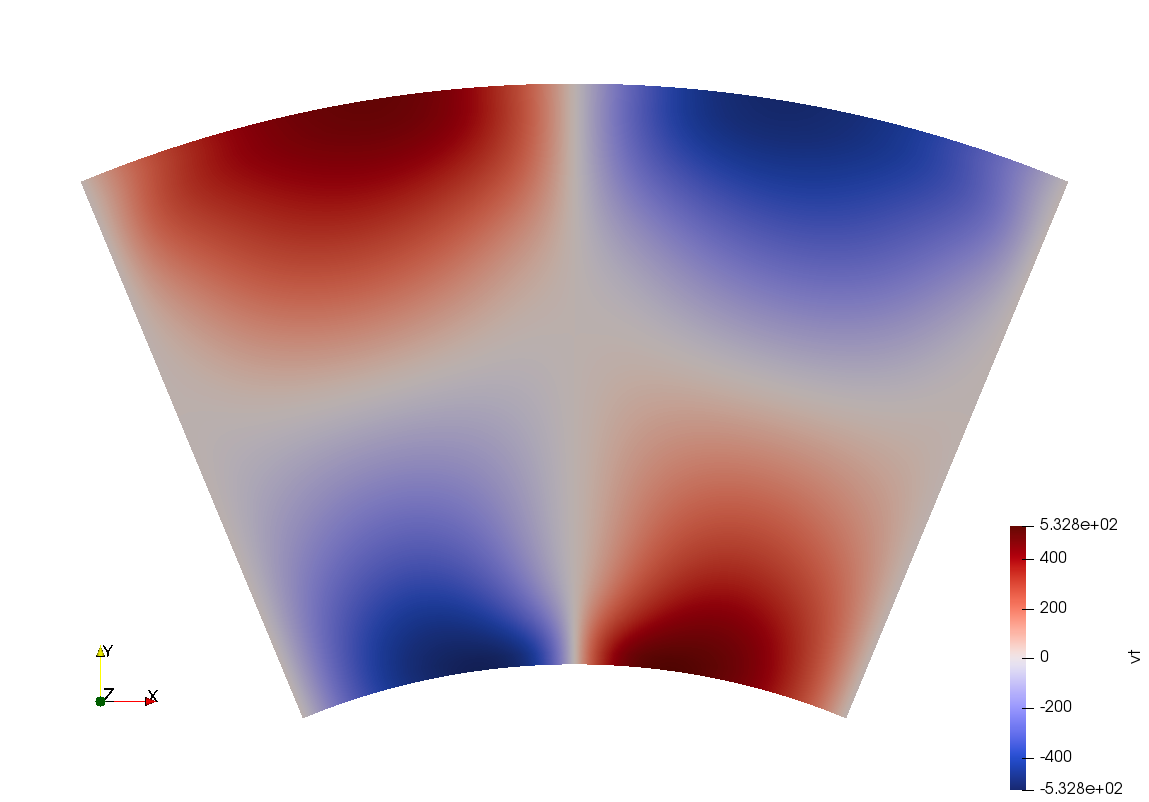
\includegraphics[width=5cm]{python_codes/fieldstone_106/results/exp2/nelr24/vt}

show viscosity, between 1 and 10!

\newpage
%%%%%%%%%%%%%%%%%%%%%%%%%%%%%%%%%%%%%%%%%%%%%%%%%%%
\subsubsection*{Strongly temperature-dependent model}
\begin{center}
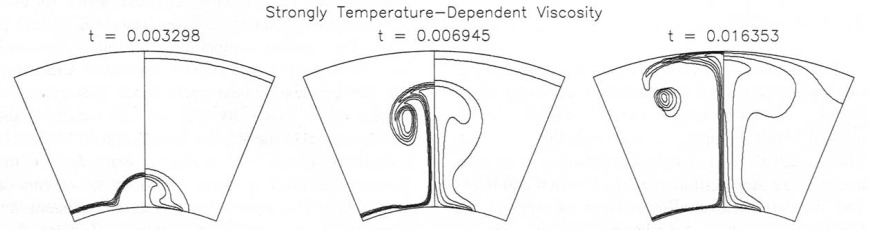
\includegraphics[width=15cm]{python_codes/fieldstone_106/images/keki97d}
\end{center}

\begin{center}
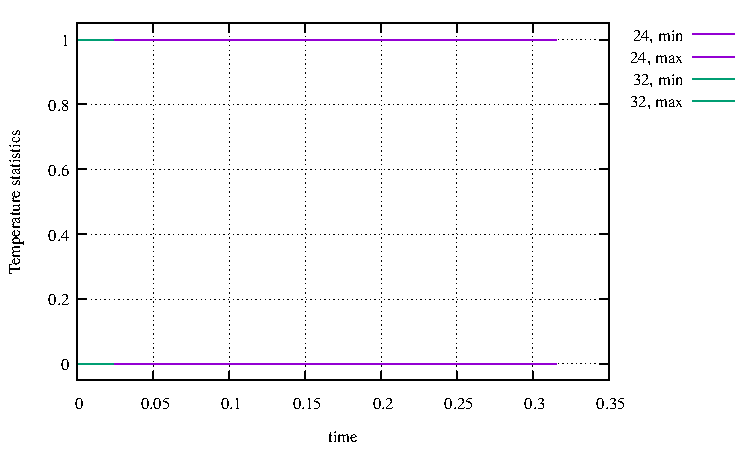
\includegraphics[width=5cm]{python_codes/fieldstone_106/results/exp3/stats_T.pdf}
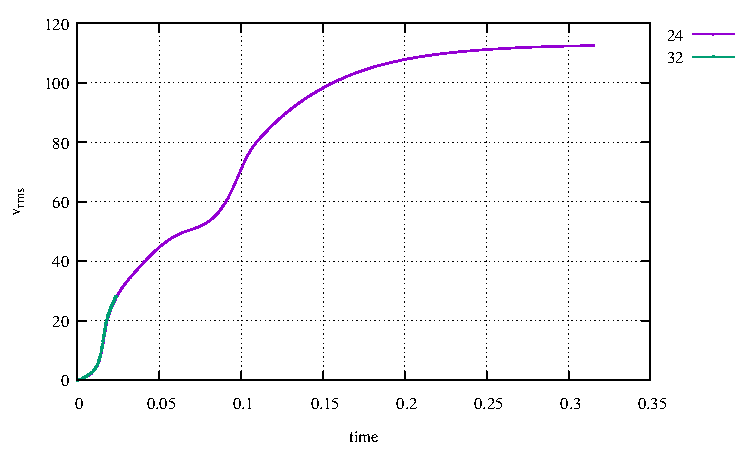
\includegraphics[width=5cm]{python_codes/fieldstone_106/results/exp3/vrms.pdf}\\
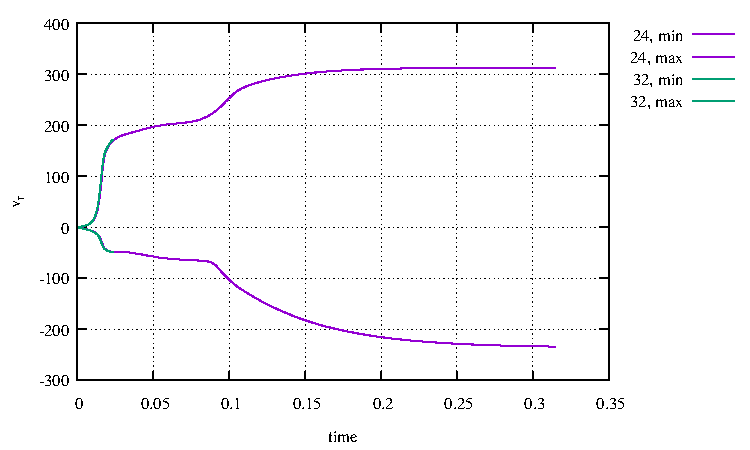
\includegraphics[width=5cm]{python_codes/fieldstone_106/results/exp3/stats_vr.pdf}
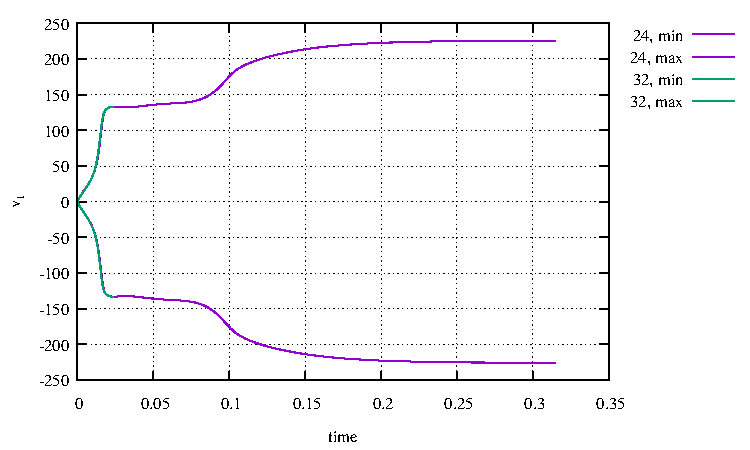
\includegraphics[width=5cm]{python_codes/fieldstone_106/results/exp3/stats_vt.pdf}\\
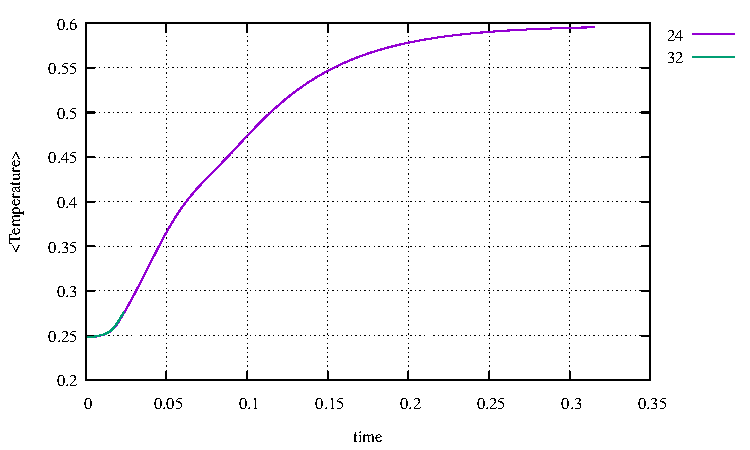
\includegraphics[width=5cm]{python_codes/fieldstone_106/results/exp3/Tavrg.pdf}
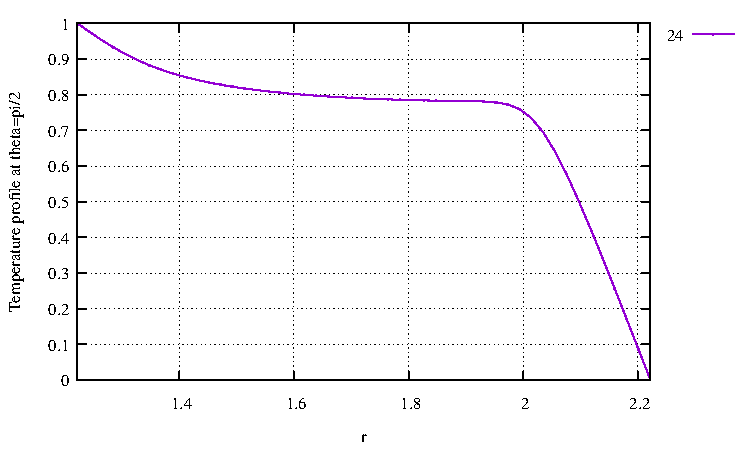
\includegraphics[width=5cm]{python_codes/fieldstone_106/results/exp3/profile_T.pdf}\\
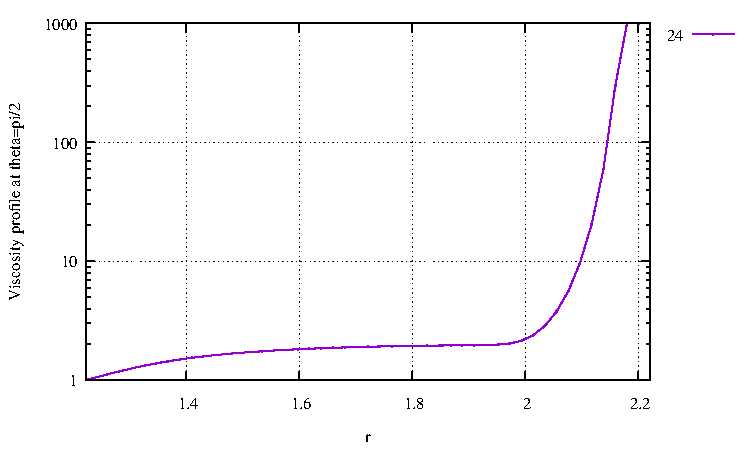
\includegraphics[width=5cm]{python_codes/fieldstone_106/results/exp3/profile_eta.pdf}\\
{\captionfont Note that none of the runs actually reached steady state. Also 
profiles are therefore not reliable.} 
\end{center}

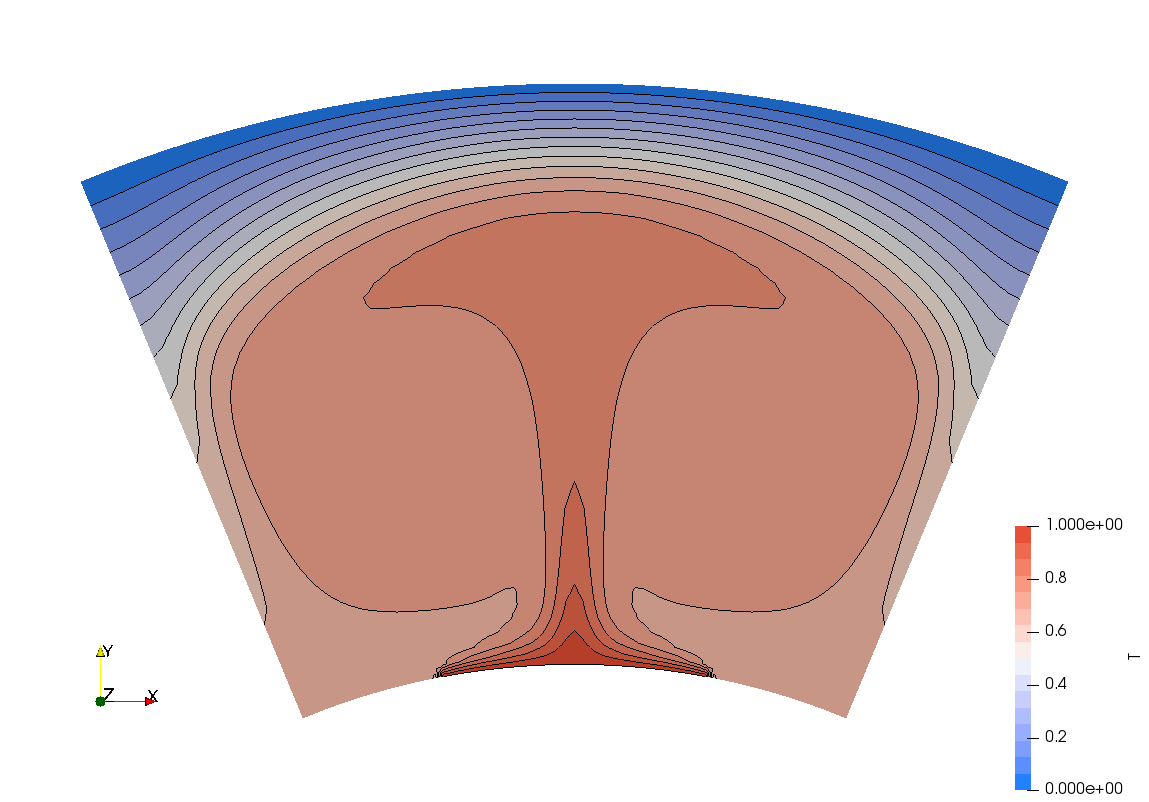
\includegraphics[width=5cm]{python_codes/fieldstone_106/results/exp3/nelr24/T}
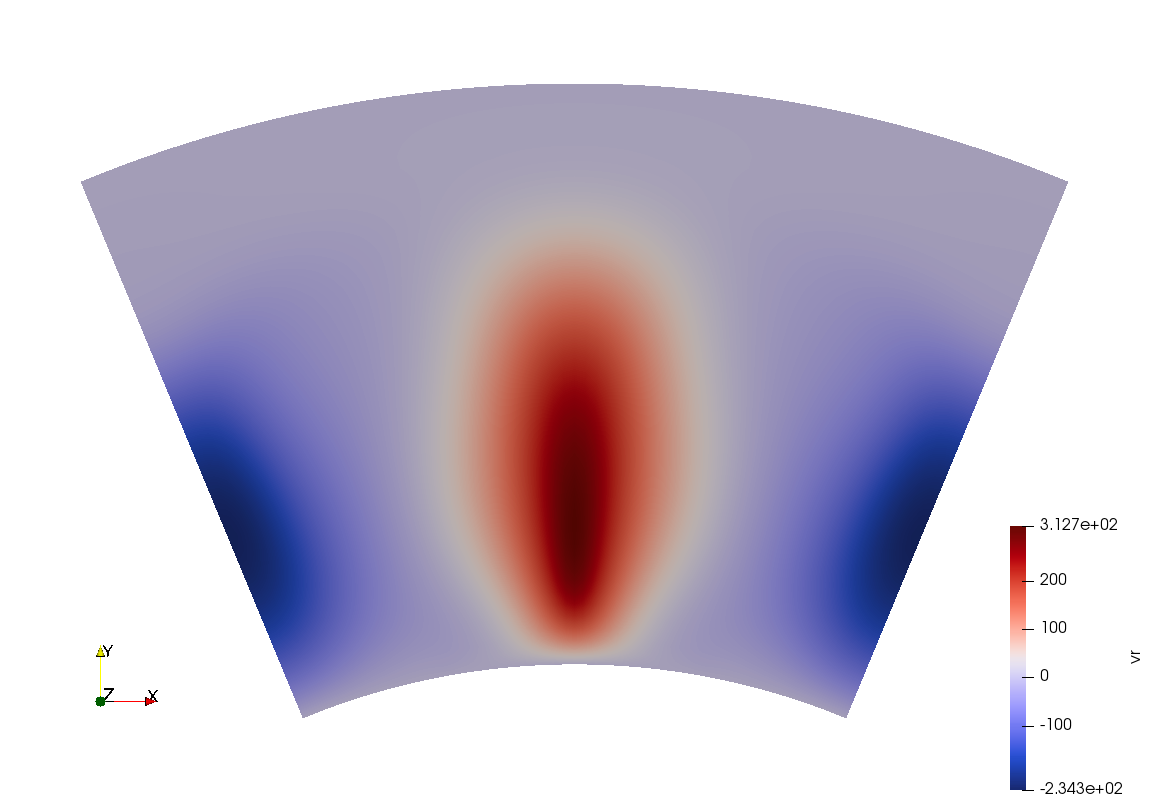
\includegraphics[width=5cm]{python_codes/fieldstone_106/results/exp3/nelr24/vr}
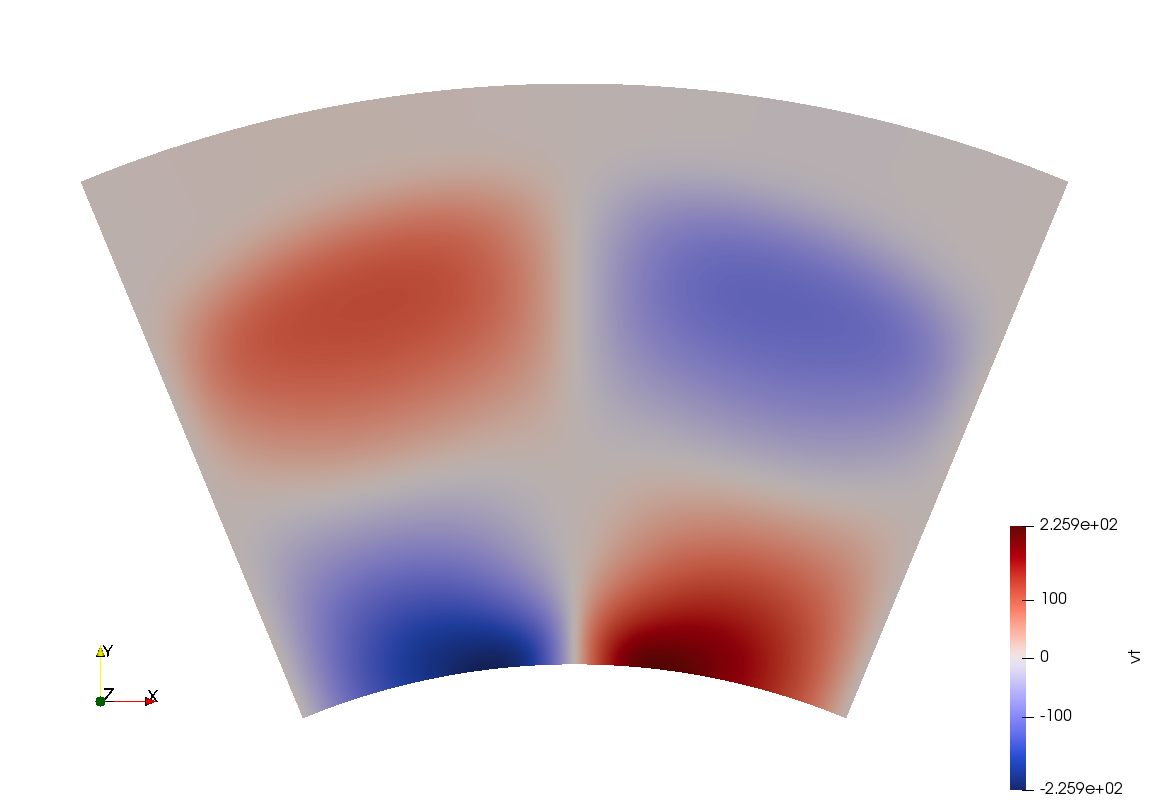
\includegraphics[width=5cm]{python_codes/fieldstone_106/results/exp3/nelr24/vt}
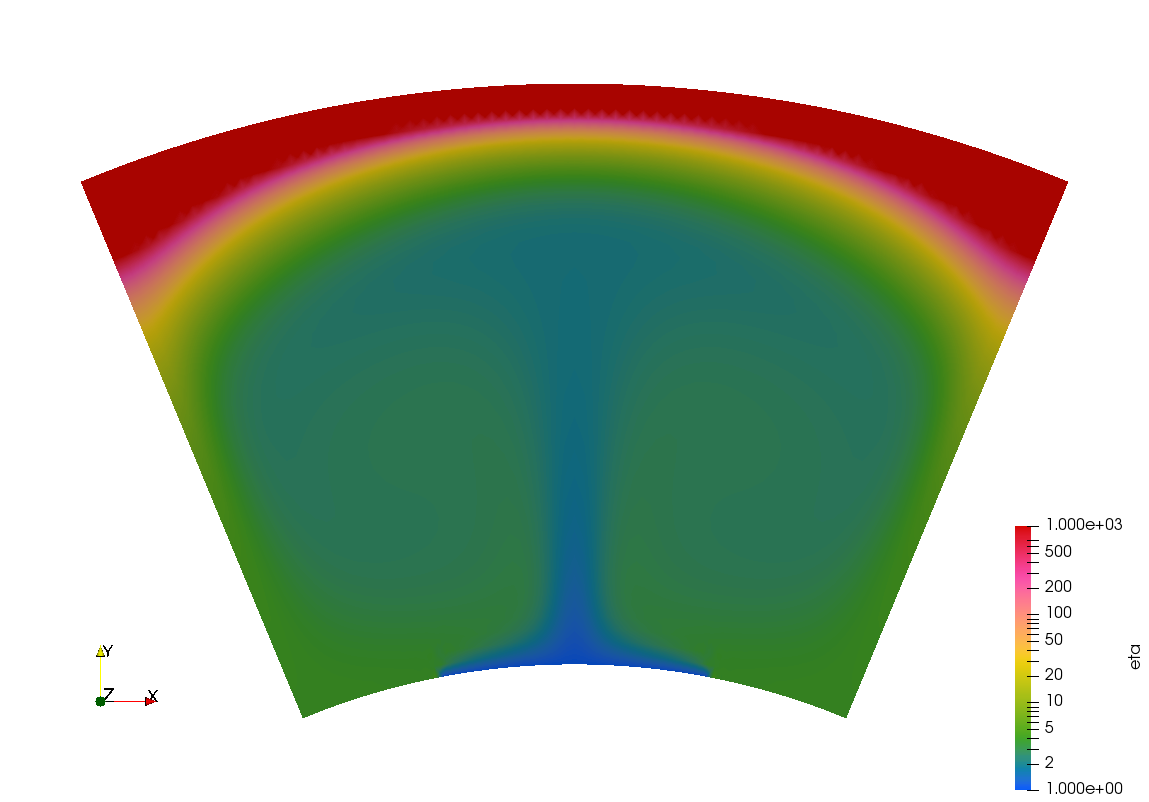
\includegraphics[width=5cm]{python_codes/fieldstone_106/results/exp3/nelr24/eta}







\newpage
What follows is an attempt at using the regular equations with Earth-like values for parameters...

The Rayleigh number is defined by
\[
\Ranb 
= \frac{\rho_0 g \alpha \Delta T (R_{outer}-R_{inner})^3}{\eta_0 \kappa}
=\frac{\rho_0^2 C_p g \alpha \Delta T (R_{outer}-R_{inner})^3}{\eta_0 k}
\]
The original article relies on dimensionless mass, momentum and energy conservation equations
but does not provide enough information to attempt an identical replication. I therefore 
choose here parameters which yield the same Rayleigh number $\Ranb=10^7$:
\begin{itemize}
\item $\rho_0=3300\si{\kg\per\cubic\metre}$
\item $\alpha=3\cdot 10^{-5} \si{\per\kelvin}$
\item $\Delta T=3000\si{\kelvin}$
\item $R_{inner}=3480\si{\km}$
\item $R_{outer}=6371\si{\km}$
\item $k=3$
\item $C_p=1250$
\item $g=9.81\si{\metre\per\square\second}$
\end{itemize}
The viscosity is then 
\[
\eta_0
=\frac{\rho_0^2 C_p g \alpha \Delta T (R_{outer}-R_{inner})^3}{\Ranb k}
\simeq 9.66 \cdot 10^{21}\si{\pascal\second}
\]
The domain is a section of an annulus with an angular opening of $\pi/4$. 
It is centered around the vertical axis. 



The viscosity is either constant ($\eta_0$) or temperature-dependent 
\[
\eta(T')
=\eta_0 \exp\left[ \frac{E}{R \Delta T} \left( \frac{1}{T'+t_0} -\frac{1}{1+t_0}  \right)   \right]
=\eta_0 \exp\left[ \frac{E}{R} \left( \frac{1}{T' \Delta T  +t_0 \Delta T} -\frac{1}{\Delta T +t_0 \Delta T}  \right)   \right]
\]
where ``$t_0$ is the surface temperature $T_{surf}$ divided by 
the temperature drop across the shell $\Delta T$'', and 
I think the authors took 
\[
T'=\frac{T-T_s}{T_p-T_s}= \frac{T-T_s}{\Delta T}
\]
\[
\eta(T)
=\eta_0 \exp\left[ \frac{E}{R} \left( \frac{1}{T-T_s  + T_s} -\frac{1}{T_p-T_s + T_s}  \right)   \right]
=\eta_0 \exp\left[ \frac{E}{R} \left( \frac{1}{T} -\frac{1}{T_p}  \right)   \right]
\]
so that $\eta(T_p)=\eta_0$. 
The authors investigate three cases:
\[
\frac{E}{R \Delta T} = \{0,0.25328,3\}
\]
With $R=8.31$ and $\Delta T=3000$ then $E=\{ 0, 6317.6 , 74829.6 \}$.
As in the paper, the viscosity is ``clipped'' to $1000\eta_0$.



